\documentclass[../main/report.tex]{subfiles}
\begin{document}

\section{Clocks}
Both the MCU and the FPGA need an external clock.
According to the design consideration AN0002 \cite{efm32gg-design-consideration})MCU need two crystals, a low frequency crystal at 32.768kHz and a high frequency crystal at 48MHz. 
For the FPGA, an oscillator of 120MHz was chosen. The frequency of the oscillator depends on the requirement of the architecture.
As seen on figure \ref{fig:oscillator-scope}, the measured period of the oscillator, with a ruler, is around $8.5 ns$, which translates to around 118 MHz.
The tolerance of the oscillator is up to 100 ppm, see datasheet \cite{xpresso-oscillator}.
Since using a ruler as a mesure tool will give unreliable results, one can assume the oscillator gives the correct output.

\begin{figure}[H]
    \centering
    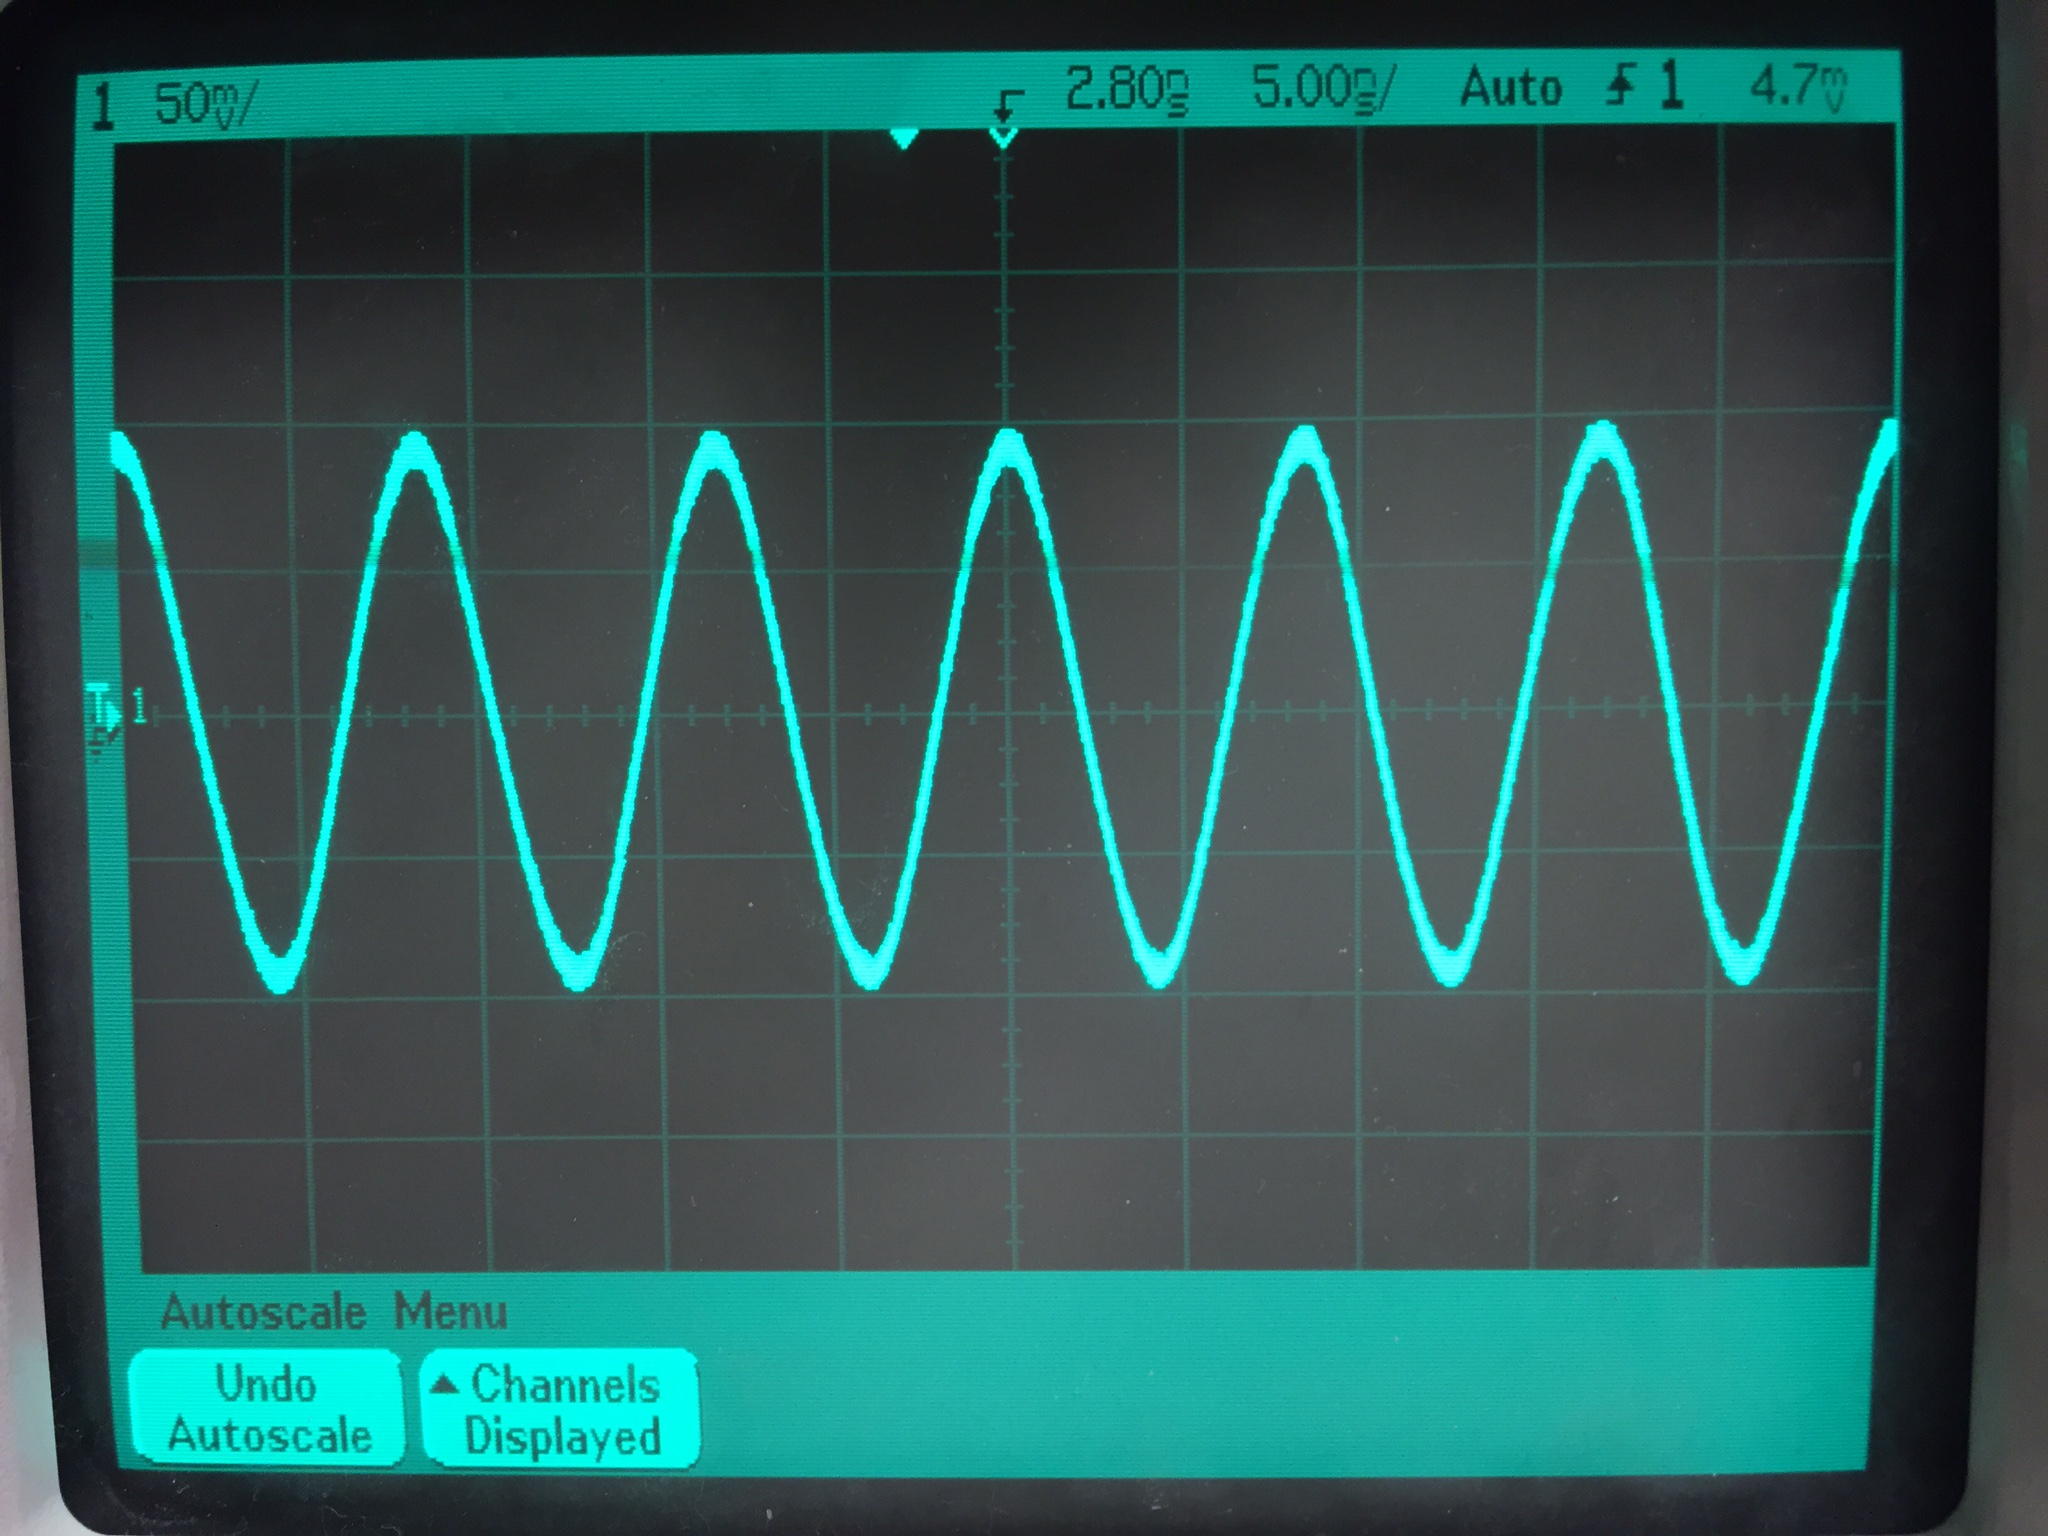
\includegraphics[width=0.85\textwidth]{../pcb/assets/oscillator.jpg}
    \label{fig:oscillator-scope}
    \caption{The oscillator on an oscilloscope.}
\end{figure}

Headers are placed between the oscillator and the FPGA. 
The headers serve as a backup in case an external oscillator is needed and act as a debugging tool.
The microcontroller clocks on the other hand have a backup solution in that the microcontroller has internal RC-oscillators for use in case the crystals malfunction.

\end{document}
